%%--------------------------------------------------------------------------
%% Lego Digital Sonoro 2 Tech Doc
%%--------------------------------------------------------------------------


\documentclass[12pt]{report}
\usepackage[utf8]{inputenc}
\usepackage{graphicx}
\usepackage{hyperref}
\usepackage{fancyhdr}
\usepackage[italian]{babel}
\usepackage{listings}
\usepackage{color}

\pagestyle{fancy}

\definecolor{dkgreen}{rgb}{0,0.6,0}
\definecolor{gray}{rgb}{0.5,0.5,0.5}
\definecolor{mauve}{rgb}{0.58,0,0.82}
\definecolor{light-gray}{gray}{0.95}
\definecolor{yellow}{RGB}{255, 251, 140}

% defining single line code blocks with monospace font and light-gray backgound (StackOverflow style)
\newcommand{\code}[1]{\colorbox{light-gray}{\texttt{#1}}}
% note command
\newcommand{\todo}[1]{\colorbox{yellow}{\textbf{\#TODO} #1}}


\lstset{frame=tb,
  language=Java,
  aboveskip=3mm,
  belowskip=3mm,
  showstringspaces=false,
  columns=flexible,
  basicstyle={\small\ttfamily},
  numbers=none,
  numberstyle=\tiny\color{gray},
  keywordstyle=\color{blue},
  commentstyle=\color{dkgreen},
  stringstyle=\color{mauve},
  breaklines=true,
  breakatwhitespace=true
  tabsize=3
}


\graphicspath{ {images/} }

\begin{document}

%!TEX root = ../main.tex
%%--------------------------------------------------------------------------
%% PAGE TITLE
%%--------------------------------------------------------------------------


\begin{titlepage}
	
    \begin{center}
    
		
\includegraphics[width=1\textwidth]{polimi.jpg}

        \vspace*{3cm}
        
        
        \Huge
        \textbf{S}ecurity \textbf{B}adge \textbf{M}anager
        
        \vspace{0.5cm}
        \LARGE
        User manual
        
        \vspace{1.5cm}
        
        \textbf{Giacomo Bresciani}
        
        \vfill
        
        
        \vspace{0.8cm}
        
        
        \Large
        Design and Implementation of Mobile Applications\\
        Prof. Luciano Baresi\\
        Politecnico di Milano\\

        
        
    \end{center}
\end{titlepage}


\tableofcontents

%!TEX root = ../Documentazione.tex
%%--------------------------------------------------------------------------
%% INTRODUCTION
%%--------------------------------------------------------------------------



\chapter{Introduzione}


\section{Scopo del documento}
Lo scopo di questo documento è quello di mostrare le scelte implementative fatte durante lo sviluppo dell'applicazione \textit{Lego Digital Sonoro 2}. Esso si divide in 4 sezioni principali: \textit{Database}, \textit{Logica di gioco}, e \textit{Interfaccia Utente}.

\section{Descrizione dell'applicazione}
\textit{Lego Digital Sonoro 2} è un videogioco per piattaforma Android progettato esclusivamente per dispositivi tablet. Lo scopo del gioco è quello di comporre parole a partire da tessere colorate rappresentanti diverse sillabe. Ogni tessera ha un colore associato direttamente alla sillaba che rappresenta e non appena viene toccata il dispositivo riproduce (tramite il sintetizzatore vocale) il suono della sillaba. Toccando due tessere una dopo l'altra è possibile comporre una parola che, se corretta, verrà aggiunta all'elenco delle parole trovate sotto forma di immagine composta dalle due tessere. La schermata consente inoltre di riascoltare le parole trovate, sia in italiano sia in inglese. Una partita può essere composta da più schermata; ogni schermata termina quando sono state trovate tutte le parole componibili con le sillabe mostrate (2 o 4).\\
Durante il corso della partita l'applicazione registra i tempi in cui vengono identificate le parole, e le invia ad una mail configurabile nelle impostazioni.\\
E' presente inoltre una modalità cooperativa a due giocatori a turni. Ogni turno consente ad un giocatore un tentativo per indovinare una parola.
%!TEX root = ../Documentazione.tex
%%--------------------------------------------------------------------------
%% DATABASE
%%--------------------------------------------------------------------------



\chapter{Database}

\section{Struttura}
\label{structure}
Il database SQLite è stato implementato tramite SugarORM, un ORM (Object-Relational Mapping) sviluppato appositamente per Android. In questo modo le entità del database sono direttamente mappate su classi Java, utilizzando il pattern DAO (Data Access Object).\\
Il database contiene 5 entità all'interno del package \\\code{it.gbresciani.legodigitalsonoro.model}:
\begin{description}
	\item[\code{Word}] Contiene la parola, sia in italiano sia in inglese, e le sillabe che lo compongono.
	\item[\code{Syllable}] Contiene la sillabla e l'esadecimale del colore associato.
	\item[\code{WordStat}] Permette di tracciare il momento in cui una parola viene trovata.
	\item[\code{GameStat}] Contiene le statistiche di una particolare partita
\end{description}
In figura \ref{fig:entities} sono riportati dettagli delle entità.

\begin{figure}[h!]
\label{fig:entities}
  \centering
    \centering{
      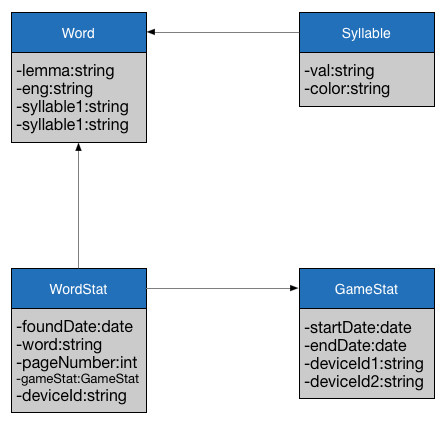
\includegraphics[width=\textwidth]{entities.png}}
  \caption{Entità presenti nel database}
\end{figure}

\section{Inizializzazione}
Il database viene inizializato la prima volta che l'applicazione viene aperta con i dati in formato \textit{JSON} presenti nei files \code{words.json} e \code{syllable.json} contenuti nella cartella degli \code{assets}.\\
Il listing \ref{lst:words_json} contiene un estratto del file \code{words.json}

\begin{lstlisting}[float, caption=Porzione del file \code{words.json}, label=lst:words_json]
[
  {
    "lemma":"arco",
    "eng":"arc",
    "syllable1":"ar",
    "syllable2":"co"
  },
  ...
\end{lstlisting}

Il mapping degli elementi JSON con la classe Java associata avviene tramite la libreria Open Source GSON, sviluppata da Goolge, che fa uso di annotazioni per mappare gli attributi delle classi con i campi JSON.\\
L'operazione di conversione dei dati da JSON a classi Java e il successivo inserimento all'interno del database, in quanto operazioni relativamente lunghe, non vengono eseguite all'interno del \textit{Thread} principale ma in uno differente grazie ad un \code{IntentService} contenuto in \\\code{it.gbresciani.legodigitalsonoro.services.InitDBService}. 


%!TEX root = ../Documentazione.tex
%%--------------------------------------------------------------------------
%% LOGICA DI GIOCO
%%--------------------------------------------------------------------------



\chapter{Logica di gioco}

La logica di gioco è affidata all'Activity \code{PlayActivity}; essa gestisce inoltre i \code{Fragments} (vedi capitolo \ref{chap:ui}) che visualizzano l'Intefaccia Utente.

\section{Glossary}
\label{sec:glossary}
In questa sezione vengono descritti acuni termini utili alla comprensione delle successive sezioni.

\begin{description}
\item[Page] Una partita è composta da una o più pagine. Una pagina può contenere 2 o 4 sillable e da 1 a 4 parole da trovare
\item[User role] Durante una partita multi player i giocatori si distinguono in ``master'', colui che ``orchestra'' la partita, e ``slave'', colui che vi partecipa in modo passivo 
\item[Turno] Durante una partita multi player rappresenta la possibilità per un giocatore di provare a indovinare una parola. Il giocatore che non è in possesso del turno attende la mossa dell'altro
\end{description}

\section{Event Bus}
\label{sec:event_bus}
Per far comunicare i vari componenti dell'applicazione (\code{Activities}, \code{Fragments}, \code{Services}) è stato utilizzato Otto\footnote{\todo{Link}}, un \textit{Event Bus}, sviluppaato appositamente per Android, che permette ai vari componenti di postare eventi su un unico Bus e per riceverli in modo asincrono.\\
La classe \code{BusProvider} permette, tramite un metodo statico, di accedere allo stesso Bus in ogni punto dell'applicazione.\\
All'interno del package \code{package it.gbresciani.legodigitalsonoro.events;
} son presenti numerose classi (ad esempio \code{WordClickedEvent} o \code{PageCompletedEvent}) che rappresentano i diversi eventi generati e ``ascoltati'' dai componenti dell'app.\\
La classe \code{NineBus} è una piccola estensione del Bus predefinito di Otto che permette tutti gli eventi sul \code{Main Thread}, anche se generati in un altro \code{Thread}.

\section{GameState}
\label{sec:game_state}
\code{GameState} è la classe che rappresenta lo stato di una partita, sia essa single o multi player. Viene inizializzato da \code{PlayActivity}, e aggiornato durante il corso della partita in seguito ai diversi eventi prodotti dagli altri componenti dell'app.\\
I suoi attributi sono:
\begin{description}
    \item[pageNumber] Il numero di pagina corrente
    \item[pages] Il numero di pagine totali della partita in corso (stabilito nelle impostazioni)
    \item[pageWordsToFindNum] Il numero di parole ancora da trovare nella pagina corrente
    \item[wordsAvailable] Un \code{ArrayList} contentente le parole ancora da trovare
    \item[wordsFound] Un \code{ArrayList} contenente le parole gia trovate
    \item[syllables] Un \code{ArrayList} contenente le syllabe presenti nella pagina corrente
    \item[currentPlayer] Se la partita è multi player contiene una stringa che rappresenta il ruolo del giocatore che detieni in quel momento il turno
    \item[currentPlayerDeviceId] Se la partita è multi player contiene una stringa che rappresenta il id del device che detieni in quel momento il turno
\end{description}

La classe \code{GameState} contiene attributi annotati con \code{@SerializedName} in modo da poter essere convertita in un oggetto JSON (tramite GSON) ed essere inviata al secondo giocatore nel caso di partita multiplayer (maggiori dettagli nella sezione \ref{sec:multiplayer}).

\section{Statistiche di gioco}
\label{sec:stats}
Le satistiche della partita, come accennato nel capitolo sul database, vengono salvate tramite i DAO \code{WordStat} e \code{GameStat} che contengono, ad esempio, i tempi di ritrovamento delle parole, le parole stesse, la pagine su cui sono state trovate o eventualmente l'id del giocatore che le ha trovate.

\section{Game flow}
\label{sec:game_flow}
Tutta le fasi di una partita sono gestite dall'\code{Activity} \code{PlayActivity}.
All'avvio, cioè durante la chiamata al metodo \code{onCreate()} essa esegue le seguenti operazioni:
\begin{enumerate}
\item Carica i settaggi della partita
\item Carica i suoni di gioco
\item Istanziaril sintetizzatore vocale \code{TextToSpeech}
\item In base al tipo di partita (single o multi player) inizializza o meno il Bluetooth e setta la variabile \code{multi} a ``MASTER'' o ``SLAVE''
\end{enumerate}

I principali metodi di \code{PlayActivity} sono:
\begin{description}
\item[\code{startGame()}] Si occupa di inizializzare gli oggetti per le statistiche e chiama \code{constructPage()} and \code{startPage()}
\item[\code{constructPage()}] Inizializza lo stato della partita (\code{GameState}) con i dati relativi alla pagina corrente. Chiama i metodi accessori \code{Helper.chooseSyllables()} (sceglie in modo casuale le sillabe per la pagina) e \code{Helper.permuteSyllablesInWords()} (calcola le permutazione delle sillabe scelte per trovare le parole componibili)
\item[\code{startPage()}] Inizializza i \code{Fragments} che mostreranno l'interfaccia utente
\item[\code{updateState()}] Si occupa di gestire la logica di gioco: determina se tutte le parole sono state trovate o se interrompere il gioco quando non è il proprio turno e posta sul Bus l'evento \code{StateUpdatedEvent} in modo che i \code{Fragments} possano reagire correttamente
\end{description}

L'\code{Activity} presenta inoltre diversi metodi annotati con \code{@Subscribe} che permettono di reagire agli eventi postati da altri componenti.

\section{Invio statistiche}
\label{sec:stats_send}
L'invio delle statistiche avviene tramite l'invio di una mail all'indirizzo settato nelle impostazioni dell'applicazione.\\
L'invio è gestito dall'\code{IntentService} \code{GenericIntentService} al quale viene passato l'id corrispondente alla partita appena conclusa. Interrogando il database esso carica i dati e li inserisce nel corpo dell'email formattandoli come mostrato nel listing \ref{lst:stats}. Il listing \ref{lst:stats_example} ne mostra invece un esempio.

\begin{lstlisting}[float, caption=Struttura delle satistiche inviate, label=lst:stats]
Dispositivo N: device id
Tempo totale: mm:ss
N - word: mm:ss (# of page on which the word was found)
...
\end{lstlisting}


\begin{lstlisting}[float, caption=Esempio di statistiche, label=lst:stats_example]
- One player -

Dispositivo 1: BC:20:A4:73:6B:49
Tempo totale: 00:13
2 - fumo: 00:02 (1)
1 - muro: 00:13 (2)

- Two Player -

Dispositivo 1: BC:20:A4:73:6B:49
Dispositivo 2: D4:0B:1A:15:FD:AD
Tempo totale: 00:14
2 - ceno: 00:02 (1)
1 - noce: 00:09 (1)
2 - buco: 00:14 (2)
\end{lstlisting}

\section{Multiplayer}
\label{sec:multi_player}
Come già detto la modalità multi player segue le stesse regole di quella single player se non per il fatto che i due giocatori provano a turno ad trovare una parola.\\
La comunicazione tra i due devices avviene tramite Bluetooth. La classe che si occupa di stabilire la connessione è \code{BluetoothService}




%!TEX root = ../Documentazione.tex
%%--------------------------------------------------------------------------
%% INTERFACCIA UTENTE
%%--------------------------------------------------------------------------



\chapter{User Interface}
\label{chap:ui}

Come anticipato nel capitolo \ref{chap:game_logic}, l'interfaccia grafica del gioco è gestita quasi interamente da \code{Fragments}, che rispondono agli eventi pubblicati sul Bus dall'activity \code{PlayActivity} aggiornando i loro componenti.\\
I due principali \code{Fragments} sono \code{WordsFragment} e \code{SyllablesFragment} (vedi figura \ref{fig:fragments}), che si occupano rispettivamente di gestire la porzione di schermo contenente le parole, e la porzione contenente le sillabe disponibili.

\begin{figure}[h!]
\label{fig:fragments}
  \centering
    \centering{
      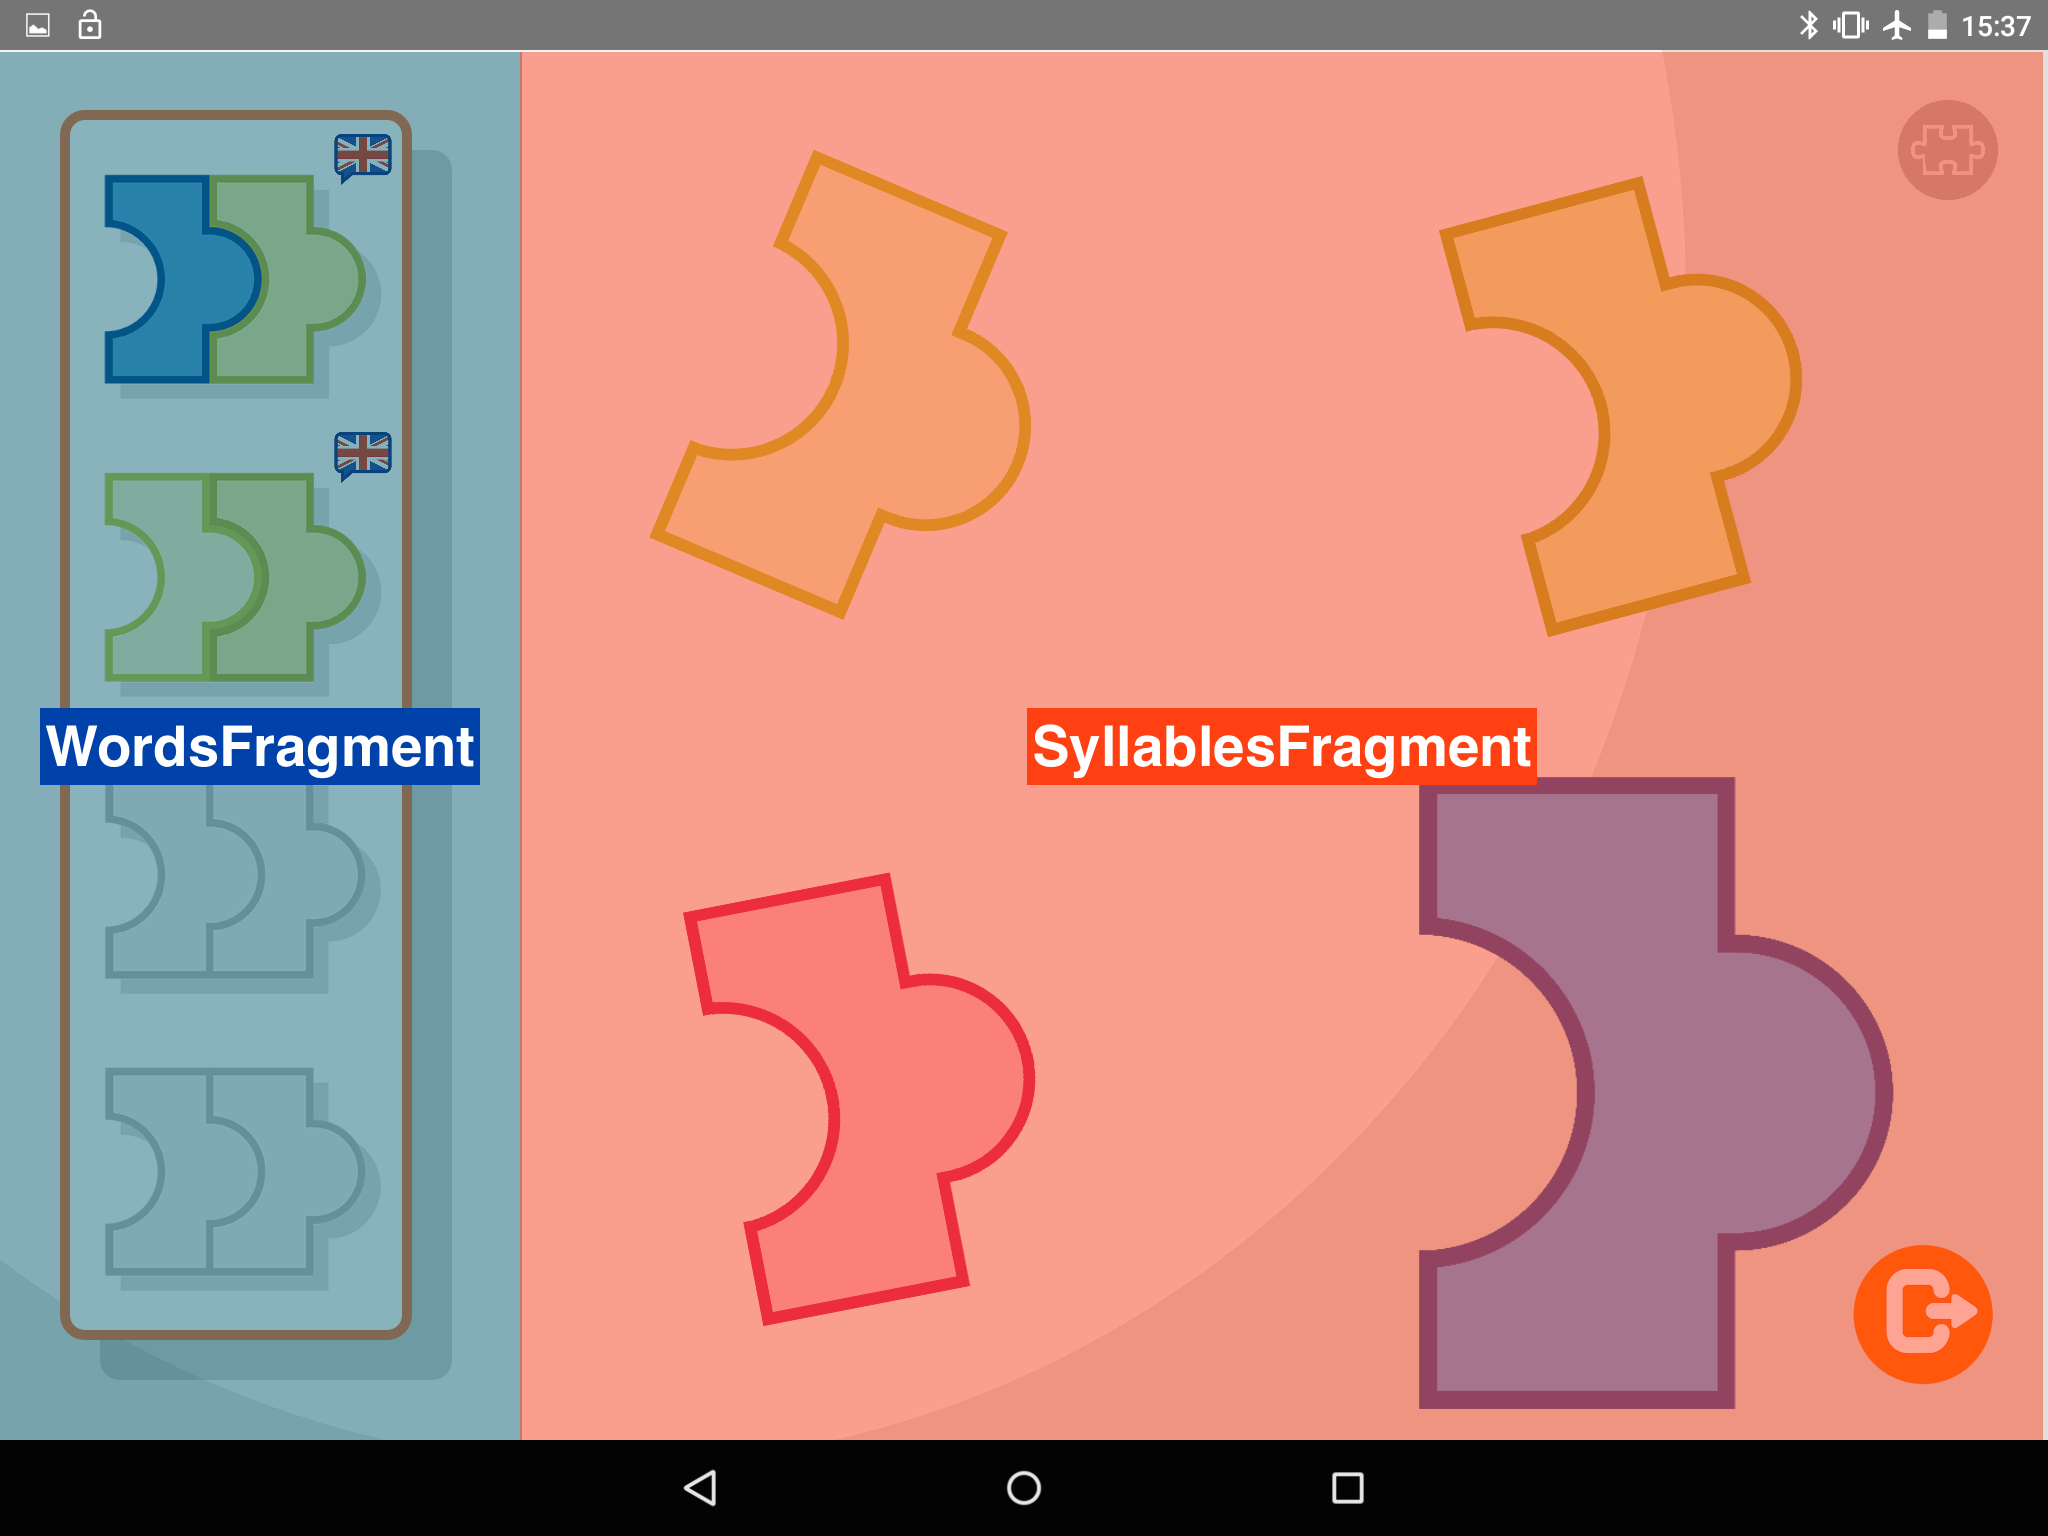
\includegraphics[width=\textwidth]{fragments.png}}
  \caption{Fragments della schermata di gioco}
\end{figure}


\section{WordsFragment}
\label{sec:words_fragment}
\code{WordsFragment} si occupa di gestire la parte di interfaccia grafica che rigurda le parole già trovate e quella ancora da trovare.\\
Esso presenta una lista verticale di ``slot'' che possono essere ``vuoti'', o ``riempiti'' con le tessere di puzzle corrispondenti alle sillabe che formano la parola. Viene inoltre mostrata accanto ad ogni slot ``pieno'' una bandiera inglese che se toccata permette di ascolare il suono della parola tradotta in inglese.\\
Il metodo \code{initUI()} si occupa, dato il numero di parole da trovare e la dimensione dello schermo (calcolata a runtime), di calcolare la dimensione degli slot corretta per gli slot con lo scompo di riempire al meglio lo spazio disponibile.\\
Le immagini degli slot sono fornite come file PNG all'interno della cartella \code{assets} e vengono caricate dinamicamente come Bitmap della dimensione corretta (per risparimare memoria) dal metodo \code{loadWordBitmap()}.\\
Il \code{Fragment} è sottoscritto all'evento \code{StateUpdatedEvent} in modo da reagire ai cambiamenti di stato della partita, come il ritrovamento di una nuova parola.

\section{SyllablesFragment}
\label{sec:syllables_fragment}

\code{SyllablesFragment} si occupa di gestire la parte di interfaccia grafica che rigurda le sillabe disponibili nella pagina corrente.\\
Esso presenta una griglia sparsa di 2 o 4 tessere di puzzle colorate rappresentanti ognuna una sillaba. Se toccate le tessere vengono selezionate e si ``alzano'' per restituire un feedback della selezione e riproducono il suono della sillaba a cui sono associate.\\
Al pari di \code{WordsFragment} calcola la dimensione corretta delle immagini e le carica come Bitmap.
%!TEX root = ../DocTecnica.tex
%%--------------------------------------------------------------------------
%% LIBRERIE
%%--------------------------------------------------------------------------



\chapter{External libraries}
They are listed here external libraries used for application development.

		\begin{description}

			\item[\href{https://github.com/emilsjolander/sprinkles}{Sprinkles}] \hfill \\
			Libreria Open Source ORM

			\item[\href{https://code.google.com/p/google-gson/}{Gson}] \hfill \\
			Java library that allows you to convert between Java objects and their representation Json.

			\item[\href{https://github.com/keyboardsurfer/Crouton}{Crouton}] \hfill \\
			Open Source library that allows to display alerts and confirmation messages.

			\item[\href{http://www.joda.org/joda-time/}{Joda-Time}] \hfill \\
			Java library for managing dates.

			\item[\href{https://try.crashlytics.com/}{Crashlytics}] \hfill \\
			Bug-tracking solution with a web inteface.

			\item[\href{https://github.com/castorflex/SmoothProgressBar}{SmoothProgressBar}] \hfill \\
			Open Source library which improves the smoothness of the default Android progressbar.

		\end{description}




\end{document}
